\section{Método proposto} \label{sec:metodo}

Nesta seção estudaremos uma estrutura em dois níveis para a complementação automática de consulta tolerante a erros que usa o algoritmo \textit{ICPAN} no primeiro nível e pesquisa tanto sequencial quanto binária no segundo nível. Para validar a ideia de busca binária no segundo nível utilizamos o ICPAN no primeiro por ser relativamente mais fácil de implementá-lo em comparação com o BEVA, que será utilizado no primeiro nível futuramente neste trabalho. O primeiro nível serve como um filtro principal que seleciona candidatos à resposta para serem processados no segundo nível, que por sua vez determina quais desses candidatos são qualificados como resposta final.

O intuito dessa abordagem é reduzir o uso de memória e ao mesmo tempo manter o desempenho quanto ao tempo de processamento da consulta. Os sistemas de busca podem se beneficiar dessa redução pois ela possibilita diminuir os custos com memória mantendo o mesmo conjunto de dados, ou então pode permitir o aumento do conjunto de dados sem que haja um grande impacto na quantidade de memória usada pelo método.

Seja $D$ a base de dados considerada nos parágrafos a seguir, composta pelos seguintes itens: \textit{\{``insects, integer, integral, integrity, intellect, intelligent, invest, invested, investigate, telepathic, telepathy, telephone, telephoto, teleport, teleprompter''\}}. Atribuímos um valor de $id$ a cada item, partindo do número $0$, como é possível observar na tabela de itens da Figura~\ref{fig:index_structure}. A etapa de indexação considera que todos os itens estão ordenados em ordem lexicográfica crescente, e para que os exemplos fiquem mais simples cada item contém apenas uma palavra.
 
\subsection{Indexação} 
\label{sec:indexing}
Seja $w$ a cadeia de caracteres de um item, e $|w|$ o tamanho da cadeia, e $w[i]$ uma indicação do $i$-ésimo caractere de $w$, começando a partir de $1$. Assim, $w[i..j]$ representa uma subcadeia de caracteres de $w$ começando na $i$-ésima posição e terminando na $j$-ésima. Consideramos também que se $j > |w|$, então $w[i..j] = w$. Seja também $\lambda$ a altura máxima permitida para a \textit{trie} $\Upsilon$, considerando que o nível do nó $\epsilon$ (nó $N0$ na Figura~\ref{fig:index_structure}) é igual a $0$. Dessa forma, o nó $N7$ tem altura igual a $3$, por exemplo. 

$\mathcal{T}$
 
 \begin{figure} [ht]
    \centering
    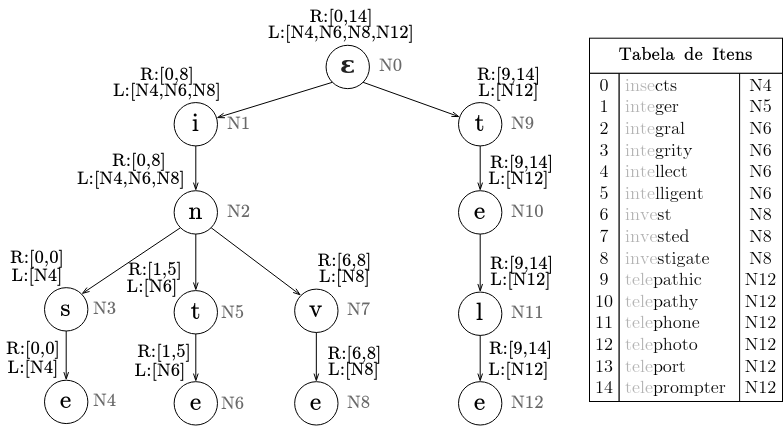
\includegraphics[width=0.94\textwidth]{figures/index-structure.png}
    \caption{Árvore \textit{trie} com os prefixos de tamanho $\lambda$ indexados, com intervalos $R$ de \textit{ids} e listas $L$ de nós folha.}
    \label{fig:index_structure}
\end{figure}

 
Como parte da implementação da estrutura proposta, indexamos as descrições textuais dos itens em uma árvore \textit{trie} $\Upsilon$ mantida em memória. Para cada cadeia $w$ de um item, inserimos em $\Upsilon$ apenas o prefixo $w[1..\lambda]$ 

Cada nó $n$ em $\Upsilon$ contém um caractere $n.caractere$, um número de identificação $n.id$, a sua altura $n.altura$ correspondente na árvore (sendo a altura do nó $\epsilon$ igual a 0), e $n.ultimo$, que é o valor do $id$ do nó folha mais à esquerda de sua subárvore, em pré-ordem. Também possui um intervalo $n.R = [menor, maior]$ no qual $menor$ e $maior$ representam respectivamente o menor e o maior $id$ dos itens em $T$ que compartilham o mesmo prefixo $p_{n}$ obtido ao caminhar partindo do nó $\epsilon$ até $n$. Para uma subárvore com raiz no nó $n$, todos os itens nessa subárvore irão compartilhar o mesmo prefixo $p_{n}$. Objetivando a simplicidade, nós nos referimos a $n$ pelo seu prefixo $p_{n}$ correspondente de forma intercambiável. 

Por fim, cada nó $n$ possui uma lista $n.L$ que contém todos os nós-folha de sua subárvore. Quando o próprio $n$ é uma folha, não possui subárvore, então a lista conterá apenas o próprio $n$, $n.L = [n.id]$.

A Figura~\ref{fig:index_structure} mostra uma \textit{trie} $\Upsilon$ após a indexação dos $\lambda = 4$ primeiros caracteres de cada item em $D$. Também mantemos uma estrutura de dicionário $H$, representada pela ``Tabela de Itens'', que mapeia o valor do \textit{id} de um item ao texto do restante da sua descrição, ou seja, $w[5..|w|]$ (texto após o 4º caractere).

Essa estrutura é utilizada para reconstruir a descrição completa de um item a partir de qualquer nó de prefixo \textit{p}. Apesar de a Figura~\ref{fig:index_structure} mostrar o texto completo de cada item, os $4$ primeiros caracteres ``apagados'' são na verdade obtidos ao caminhar por $\Upsilon$. Para possibilitar essa reconstrução, também guardamos em $H$ o $id$ do nó correspondente ao prefixo do item. Supondo por exemplo a reconstrução de ``\textit{investigate}'', com $id=7$ em $H$, basta processar o prefixo $p$ do nó $N8$, que é \textit{p = ``inve''}, como mostra a Figura~\ref{fig:index_structure}, e então concatenar $p$ com ``\textit{stigate}'', que é o conteúdo presente em $H$ para a chave $id=7$.

\subsection{Primeiro nível}
\label{sec:first-level}

O algoritmo de busca utilizado no primeiro nível será o ICPAN, proposto por Li et al. Como descrito na seção~\ref{sec:related_work} algoritmo ICPAN utiliza um algoritmo incremental que calcula os prefixos semelhantes a um prefixo consultado, tolerando uma quantidade erros de digitação previamente definida como o limite de distancia de edição $\tau$.

Uma característica desse algoritmo é a ``ativação'' de nós da \textit{trie} que correspondem a um prefixo que pode ser obtido considerando erros no prefixo consultado. Pode existir um erro, ou mais, dependendo do limite de distância de edição $\tau$ escolhido para a consulta. Para facilitar a compreensão do processo em dois níveis, faremos referências ao algoritmo~\ref{alg:2-level} nos parágrafos seguintes.

Seja $p$ um prefixo consultado pelo usuário. Considerando que $p[1..\lambda]$ é uma sub-cadeia de caracteres de $p$ que vai do 1º até o $\lambda$-ésimo caractere, e que $p[1..\lambda] = p$ se $|p| \leq \lambda$, nós processamos a subcadeia $p[1..\lambda]$ na linha $3$ com o algoritmo ICPAN caractere a caractere, de acordo com os passos do algoritmo descritos na seção~\ref{sec:second_level}. Após terminar essa etapa obtemos um conjunto $\Psi_{p[1..\lambda]} = \{ \langle n, \xi_{n}^{p[1..\lambda]}, m_{i}, \xi_{n}^{p_{i}} \rangle \}$ de \textit{nós pivô ativos de} $p[1..\lambda]$. Se $|p| \leq \lambda$ consideramos que $p$ é uma consulta ``comum'', e então realizamos o processamento caractere a caractere padrão do ICPAN para obter a resposta na linha $5$. No entanto, quando $|p| > \lambda$, é necessário dividir o processamento em dois níveis.

\begin{algorithm}[ht]
\caption{Complementação de consultas tolerante a erros em dois níveis}\label{euclid}
\label{alg:2-level}
\begin{algorithmic}[1]
\Function{processarConsulta}{$p$}
    \State $resultados \gets \emptyset$
    \State $\Psi_{p[1..\lambda]} \gets processarConsultaComICPAN(p[1..\lambda])$  \Comment{Nós pivô ativos para $p[1..\lambda]$}
    \If{$|p| < \lambda$}
        \State \textbf{return} $recuperarResultadosICPAN(\Psi_{p[1..\lambda]})$
    \EndIf
    \For{$\langle n, \xi_{n}^{p[1..\lambda]}, m_{i}, \xi_{n}^{p_{i}} \rangle \in \Psi_{p[1..\lambda]} $}
        \If{$\xi_{n}^{p[1..\lambda]} < \tau$}
            \For{$n_{folha} \in n.L$}
                \For{$itemId \in n_{folha}.R$}
                    \If{$itemId \in resultados$}
                        \State \textbf{continue}
                    \EndIf
                    \State $candidato \gets H[itemId].reconstruirTexto()$
                    \State $distancia \gets levenshtein(candidato[1..|p|], p)$ 
                    \If{$distancia \leq \tau$}
                        \State $resultados \gets resultados \cup \{ itemId \}$
                    \EndIf
                    
                \EndFor
            \EndFor
        \Else
            \For{$n_{folha} \in n.L$}
                \State $p' \gets p[\lambda+1+ (n.altura - |m_{i}|)..|p|]$
                \State $limInferior \gets buscaBinariaLimInf(p', n_{folha}.R, n.altura)$
                \State $limSuperior \gets buscaBinariaLimSup(p', n_{folha}.R, n.altura)$
                
                \If{$limInferior \ge 0$ \textbf{and} $limSuperior \ge 0$}
                    \State $i \gets 0$
                    \While{$i + limInferior \le limSuperior$}
                        \State $resultados \gets resultados \cup \{ leaf.ids[limInferior + i] \} $
                        \State $i \gets i + 1$
                    \EndWhile
                \EndIf
            \EndFor
        \EndIf
    \EndFor
    \State \textbf{return} $resultados$ 
\EndFunction
\end{algorithmic}
\end{algorithm}

\subsection{Segundo nível}
\label{sec:second_level}

O segundo nível é responsável por analisar cada prefixo de item candidato à resposta gerado no primeiro nível, e determinar quais deles são qualificados como resposta final e quais não são. Isso é feito através de dois tipos de busca: sequencial e binária. 

Cada tupla $\langle n, \xi_{n}^{p[1..\lambda]}, m_{i}, \xi_{n}^{p_{i}} \rangle$ do conjunto $\Psi_{p[1..\lambda]}$ gerado no primeiro nível é examinada, como é possível observar na linha $7$. Um nó $n$ pivô ativo de uma tupla qualquer pode ser categorizado como:
\begin{itemize}
    \item \textit{Nó de borda} -- quando $\xi_{n}^{p[1..\lambda]} = \tau$. Checagem realizada na linha $8$.
    \item \textit{Nó comum} -- quando $\xi_{n}^{p[1..\lambda]} < \tau$.
\end{itemize}

O critério considerado para determinar qual tipo de busca utilizar ao examinar os nós-folha de um nó pivô depende de sua categoria. Se for um nó comum, usamos a busca sequencial, e se for um nó de borda, a busca binária é utilizada. A seguir detalharemos as particularidades do processamento em cada uma das categorias de nó pivô.

Um nó pivô $n$ é dito comum quando a quantidade de erros entre seu prefixo e $p[1..\lambda]$ é menor que o limiar $\tau$. Isso quer dizer que ainda pode haver erros entre o restante do prefixo consultado e o restante dos textos dos itens referenciados pelo nó $n$. Esse é o caso tratado entre as linhas $9$ e $20$. Na linha $9$ ocorre uma iteração por cada nó folha $n_{folha}$ da subárvore com raiz em $n$, e na linha $10$ ocorre uma iteração para todos os \textit{ids} de itens referenciados pelo intervalo $n_{folha}.R$. Na linha $11$, é checado se o id já está no conjunto de resultados, e se estiver, seu processamento é ``pulado''. Na linha $14$ reconstruímos na variável $candidato$ o texto completo do item, com auxílio da estrutura $H$. Então, calculamos a distância de \textit{Levenshtein} na linha $15$ entre os $|p|$ primeiros caracteres do texto completo do item e a consulta de prefixo $p$. Se essa distância estiver dentro do limiar $\tau$, então o item candidato é considerado um resultado qualificado.

Já um nó pivô $n$ é um nó de borda quando a distância de edição entre seu prefixo e $p[1..\lambda]$ é exatamente o valor do limiar $\tau$. Isso quer dizer que todos os erros possíveis tolerados foram ``esgotados'' no primeiro nível, e que nesse caso é possível realizar comparações simples de texto no segundo nível. Na linha $22$ iteramos sobre todos os nós folha $n_{folha}$ da subárvore com raiz em $n$. Na linha $23$ é definido o valor $p' = p[\lambda+1+ (n.altura - |m_{i}|)..|p|]$, que será procurado com as buscas binárias. Como os itens referenciados pelos \textit{ids} presentes no intervalo $n_{folha}$ estão ordenados em ordem lexicográfica crescente, é possível realizar duas buscas binárias pelo valor de $p'$ nesse intervalo, sendo uma de limite inferior (linha $24$) e outra de limite superior (linha $25$). As duas funções de busca binária retornam $-1$ caso não o valor procurado não seja encontrado. Em seguida, é preciso checar se os dois limites são positivos na linha $26$. Caso forem, então os \textit{ids} contidos no intervalo $[limInferior, limSuperior]$ são considerados resultados qualificados.